\documentclass{article}
\usepackage[english]{babel}
\usepackage{spconf,amsmath,graphicx}
\usepackage{enumitem}
\setlist{nosep, leftmargin=14pt}
\usepackage{spconf,amsmath,graphicx,epsfig,multirow,subfigure}
\usepackage{hhline}                     % for merging cells in the table
\usepackage{array,ragged2e}     		% for aligning cells in tables
\usepackage{flushend}                   % for balancing the references
\usepackage{url}
\usepackage{dblfloatfix}
% Example definitions.
% --------------------

\usepackage{mwe} % to get dummy images

% Example definitions.
% --------------------
\def\x{{\mathbf x}}
\def\L{{\cal L}}



\newcolumntype{M}[1]{>{\centering\arraybackslash}m{#1}} % for centering all columns and rows
\newcolumntype{P}[1]{>{\centering\arraybackslash}p{#1}} % for centering all columns and rows
\newcolumntype{R}[1]{>{\raggedleft\arraybackslash}p{#1}} % for right-alignment all columns and rows
\newcolumntype{L}[1]{>{\raggedright\arraybackslash}p{#1}} % for left-alignment all columns and rows

% Commands for refer figs, eqs, and others
\newcommand{\figref}[1]{Fig.~\ref{fig:#1}}
\newcommand{\tblref}[1]{Table~\ref{tbl:#1}}
\newcommand{\eref}[1]{Eq.~\eqref{eq:#1}}
\newcommand{\secref}[1]{Section~\ref{sec:#1}}
\newcommand{\subsecref}[1]{Section~\ref{subsec:#1}}


\title{Design a neural network to generate a survival classifier for the Titanic dataset}

\name{Nguyen H. Hoang, Pham X. Cuong}
\address{Le Quy Don Technical University, Vietnam}

\begin{document}
\maketitle
\begin{abstract}
    The sinking of the Titanic is one of the most infamous shipwrecks in history.
    On April 15, 1912, during her maiden voyage, the widely considered “unsinkable” RMS Titanic sank after colliding with an iceberg.
    Unfortunately, there weren’t enough lifeboats for everyone onboard, resulting in the death of 1502 out of 2224 passengers and crew.
    In this report, we present a predictive model that answers the question: “what sorts of people were more likely to survive?” using passenger data (ie name, age, gender, socio-economic class, etc).
\end{abstract}


%-------------------------------------------------------------------------------------
% Introduction
%-------------------------------------------------------------------------------------
\section{Introduction}
\label{sec:intro}
In this report, we have gain access to two similar datasets that include passenger information like name, age, gender, socio-economic class, etc. One dataset is titled `train.csv` and the other is titled `test.csv`.
Train.csv will contain the details of a subset of the passengers on board (891 to be exact) and importantly, will reveal whether they survived or not, also known as the “ground truth”.
The `test.csv` dataset contains similar information but does not disclose the “ground truth” for each passenger. It’s your job to predict these outcomes.
Using a neural network for traning in the train.csv data, predict whether the other 418 passengers on board (found in test.csv) survived.
\begin{itemize}
    \item The dataset have \textbf{11} features: \textit{PassengerId}, \textit{Pclass}, \textit{Name}, \textit{Sex}, \textit{Age}, \textit{SibSp}, \textit{Parch}, \textit{Ticket}, \textit{Fare}, \textit{Cabin}, \textit{Embarked} and \textit{Survived}.
    The \textit{Survived} show that \textbf{2} labels Survived or not with \textbf{1} and \textbf{0}.
    \item While there was some element of luck involved in surviving,
    it seems some groups of people were more likely to survive than others.
    So we will figure out that with neural network.
    \item By using a Multilayer perceptron (MLP) neural network, we can predict the outcome of the survival of the passengers.
    \item In this report, we will show how to use the `train.csv` dataset to train a neural network and then use the trained model to predict the outcome of the survival of the passengers in the `test.csv` dataset. 
\end{itemize}

%-------------------------------------------------------------------------------------
% Proposed method
%-------------------------------------------------------------------------------------
\section{Method}

\begin{itemize}
    \item Preprocessing the data:
        \begin{itemize}
            \item In the dataset, we drop \textit{PassengerId}, \textit{Name}, and \textit{Ticket},
            Because they are unique by each passenger.
            We also drop \textit{Cabin} because total of dataset have \textbf{891} samples and \textit{Cabin} have \textbf{687} is \textbf{None}.
            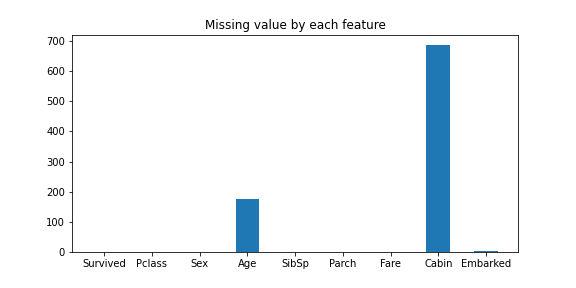
\includegraphics[width=0.425\textwidth]{missing.png}   
            \item Normalize the data, we vectorize from discrete value to unique number value and use MinMaxScaler to normalize data.
            \[
               X_{new} = \frac{X - X_{min}}{X_{max} - X_{min}}
            \]
            \item Impute the missing values in \textit{Age} and \textit{Embarked},
            we use KNN algorithm to impute the missing values with \textbf{N neighbors} is 2 and formula caculate distance is \textbf{nan euclidean distances} .
            \[
            NED(x,y) = \sqrt{\frac{S}{S_{nnan}} \sum^n_{i=0} d(x,y)^2 }  
            \]
            \item Split the data into training, testing sets and validation sets with ratio is \textbf{7}:\textbf{2}:\textbf{1}.
        \end{itemize}
    \item Build a Multilayer perceptron (MLP) neural network with the following hyperparameters:
        \begin{itemize}
            \item \textbf{Number of input layers} is \textbf{7} from the input shape of the dataset after processed.
            \item \textbf{Number of hidden layers} is \textbf{3} and \textbf{number of neurons} in each layer is \textbf{8} and activation function is \textbf{ReLU}.
            \item \textbf{Number of output layers} is \textbf{1} for classification is survival or not with \textbf{Sigmoid} activation function.
            \begin{center}
                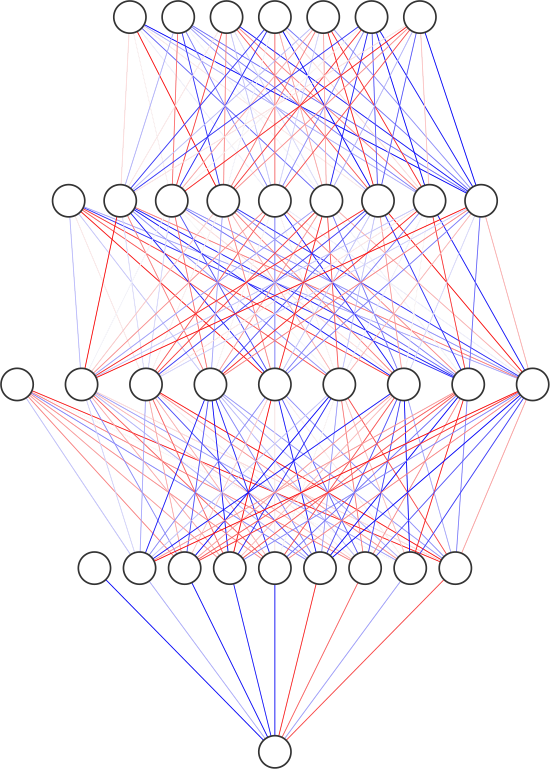
\includegraphics[width=0.235\textwidth]{nn.png}
            \end{center}
            \item We use \textbf{Adam Optimization Algorithm} for update network weights iterative based on training data.
            \begin{gather}
                g_n \gets \nabla f(\theta_{n-1})
                \\
                m_n \gets \frac{\beta_1}{1-\beta_1^n}m_{n-1} + \frac{1-\beta_1}{1-\beta_1^n}g_n
                \\
                v_n \gets \frac{\beta_2}{1-\beta_2^n}v_{n-1} + \frac{1-\beta_2}{1-\beta_2^n}g_n \odot g_n
                \\
                \theta_{n} \gets \theta_{n-1} - \alpha \frac{m_n}{\sqrt{v_n} + \epsilon}
            \end{gather}
                with \(\alpha\) is \textbf{0.001}, \(\epsilon\) is \textbf{1e-07}, \(\beta_1\) and \(\beta_2\) are \textbf{0.9} and \textbf{0.999} respectively.
        \end{itemize}
    \item This is a binary classification problem, so we use \textbf{binary cross-entropy} loss function.
    \begin{gather}
        -p(x).\log q(x) - (1-p(x)).log(1-q(x))
    \end{gather}
    with \(p(x)\) is target probability and \(q(x)\) is predicted probability.
\end{itemize}
%-------------------------------------------------------------------------------------
% Experimental results and analysis
%-------------------------------------------------------------------------------------
\section{Experimental results and analysis}
\begin{itemize}
    \item The train dataset 
        \\
        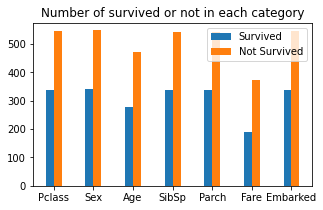
\includegraphics[width=0.425\textwidth]{chart_sur_or_not.png}
        as we can see, there are 'Not survived' more than 'Survived' by each category.
        \\
        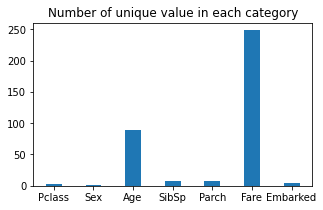
\includegraphics[width=0.425\textwidth]{chart_unique.png}   
    \item We training with \textbf{100} epochs and \textbf{batch size} is \textbf{16}.
    \item There are the best accuracy, loss, F1 score, precision, and recall on train dataset and validation dataset after train 5 times.
    \\
    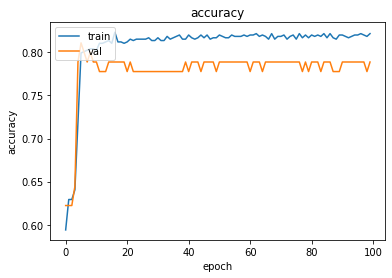
\includegraphics[width=0.425\textwidth]{accuracy.png}
    \\
    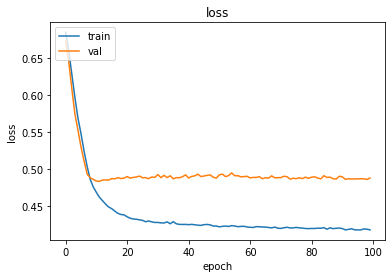
\includegraphics[width=0.425\textwidth]{loss.png}
    \\
    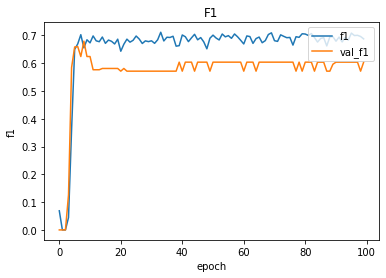
\includegraphics[width=0.425\textwidth]{f1.png}
    \\
    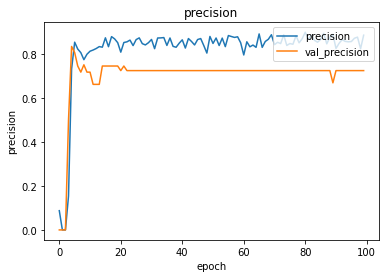
\includegraphics[width=0.425\textwidth]{precision.png}
    \\
    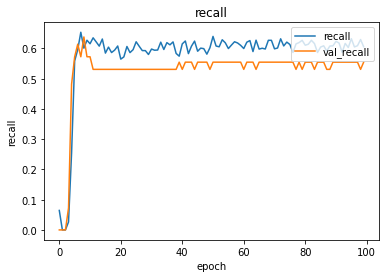
\includegraphics[width=0.425\textwidth]{recall.png}
    \\
    \item The results on test dataset.
    \\\\
    \begin{tabular}{|c|c|c|c|c|c|}
        \hline
        Train times & 1     & \textbf{2}     & 3     & 4     & 5     \\ \hline
        Accuracy    & 0.803 & \textbf{0.837} & 0.808 & 0.808 & 0.820 \\ \hline
        Loss        & 0.448 & \textbf{0.440} & 0.445 & 0.442 & 0.454 \\ \hline
        F1-score    & 0.732 & \textbf{0.778} & 0.740 & 0.730 & 0.754 \\ \hline
        Precision   & 0.843 & \textbf{0.899} & 0.859 & 0.880 & 0.868 \\ \hline
        Recall      & 0.662 & \textbf{0.694} & 0.655 & 0.637 & 0.673 \\ \hline
    \end{tabular}
    \\
    \item Because Recall is low compared to Precision, it can be seen that the model is making the choice 'Not surviverd' over 'Surviverd'.
    \item Loss is quite high at 0.44, because the sigmoid activation function is curved, it is difficult to separate clearly between 0 and 1.
\end{itemize}

%-------------------------------------------------------------------------------------
% Discussions
%-------------------------------------------------------------------------------------
\section{Conclusion}
Using neural networks to solve the problem and achieve not bad results, but there will be machine learning algorithms that give higher accuracy. Therefore, it will be necessary to improve this neural network in different ways to give better results.
%-------------------------------------------------------------------------------------
% References
%-------------------------------------------------------------------------------------
% \section{REFERENCES}
% 
% References should be produced using the bibtex program from suitable
% BiBTeX files (here: strings, refs, manuals). The IEEEbib.bst bibliography
% style file from IEEE produces unsorted bibliography list.
% -------------------------------------------------------------------------
\bibliographystyle{IEEEbib}
\label{sec:refs}
\bibliography{refs}

\end{document}
